\documentclass{beamer}

% \usepackage{beamerthemesplit} // Activate for custom appearance
\usepackage{graphicx}

\setbeamertemplate{navigation symbols}{}
\setbeamertemplate{footline}
{
    \leavevmode%
    \hbox{%
        \begin{beamercolorbox}[wd=.333333\paperwidth,ht=2.25ex,dp=1ex,center]{author in head/foot}%
            \usebeamerfont{author in head/foot}\insertshortauthor
        \end{beamercolorbox}%
        \begin{beamercolorbox}[wd=.333333\paperwidth,ht=2.25ex,dp=1ex,center]{title in head/foot}%
            \usebeamerfont{title in head/foot}\insertshorttitle
        \end{beamercolorbox}%
        \begin{beamercolorbox}[wd=.333333\paperwidth,ht=2.25ex,dp=1ex,right]{date in head/foot}%
            \usebeamerfont{date in head/foot}\insertshortdate{}\hspace*{2em}
            \insertframenumber{} / \inserttotalframenumber\hspace*{2ex} 
        \end{beamercolorbox}}%
        \vskip0pt%
    }

\title{Kernel Panic}
\author{Gruppe 09}
\date{23.05.2019}

\begin{document}


{
\usebackgroundtemplate{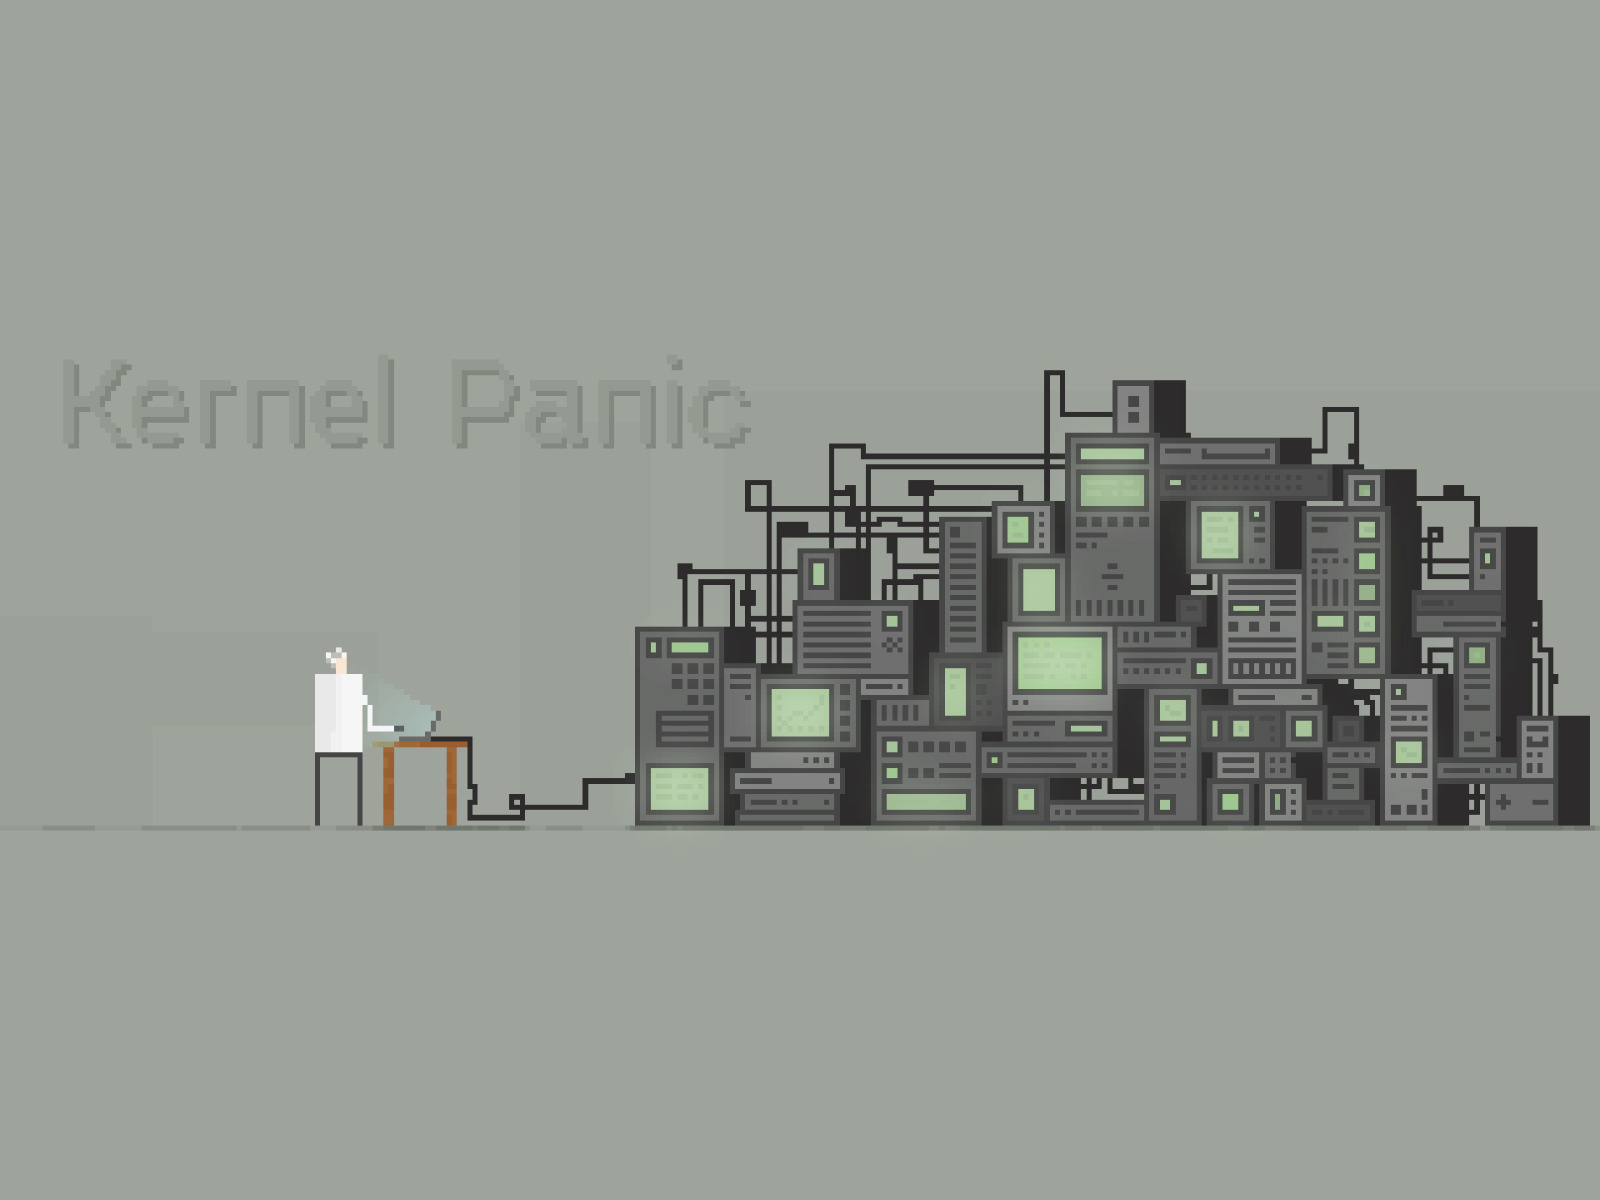
\includegraphics[width=\paperwidth]{kernel-panic-4-3.png}}
\frame{}
}

\section[Outline]{}
\frame{\tableofcontents}

\section{Spielkonzept}
\begin{frame}
\frametitle{\secname}
\begin{itemize}
\item Mischung aus Tower Defense und MOBA
\item Man spielt gegen eine KI
\item 2 Lanes, je eine für Angriff und Abwehr
\item Ziel ist es möglichst oft an die gegnerische Basis zu gelangen
\end{itemize}
\end{frame}

\begin{frame}
\frametitle{Abwehr}
\begin{itemize}
\item Kabel um den Weg zu versperren
\item CD Werfer schießt auf den Gegner
\item Lüftung verlangsamt Einheiten
\item usw.
\end{itemize}
\end{frame}

\begin{frame}
\frametitle{Angriff}
\begin{itemize}
\item Angriffswellen:
\begin{itemize}
\item nicht steuerbare Einheiten
\item z.B. Virus oder Trojaner
\end{itemize}
\item Helden:
\begin{itemize}
\item sind nicht von Wellen abhängig
\item können gezielt gesteuert werden
\item z.B. Firefox, der Gebäude überspringen kann
\end{itemize}
\end{itemize}
\end{frame}

\begin{frame}
\frametitle{Upgrades}
\begin{itemize}
\item geteilter Fähigkeitenbaum in der Mitte
\item verbessert z.B Effizienz der Türme und Angriffseinheiten oder Anzahl der gleichzeitig verfügbaren Helden
\item kostet Erfahrungspunkte, welche durch Besiegen gegnerischer Wellen erspielt werden können
\end{itemize}
\end{frame}

\section{Spielende}
\begin{frame}
\frametitle{\secname}
\begin{itemize}
\item Wenn die Ladung einer Basis auf 0\% gesunken ist
\item Gewonnen hat der Spieler dessen Basis noch Ladung hat
\end{itemize}
\end{frame}

\section{Alleinstellungsmerkmal}
\begin{frame}
\frametitle{\secname}
\begin{itemize}
\item zwei Lanes
\item gezielt kontrollierbare Helden
\item geteiltes Fähigkeitenkontingent
\end{itemize}
\end{frame}

\section{Warum macht Kernel Panic Spaß?}
\begin{frame}
\frametitle{\secname}
\end{frame}

\end{document}
